\chapter{Methods and Data}
The abundance of information of the electromagnetic spectrum allowed us to build highly detailed models of various celestial objects such as stars, both on their individual internal structure and on how this is influenced by the interaction with other bodies, for instance in binary systems.
In the pursuit of reaching a greater sensitivity in the gravitational counterpart too, which could potentially reveal new information, or place better constrains on the existing models, these stellar models, when combined with a good theory of gravity, can be used to construct synthetic populations that reproduce observable features like luminosity, color, and chemical composition, which could enable us to predict what their gravitational signal would look like.
In gravitational waves research, our observational capabilities are still very limited, and the signals are still comparatively very weak relative to their electromagnetic counterpart. 
Thererfore, methods that rely on simulations can be very useful both to  explore how different sources could look like in the gravitational wave domain, and how effectively they could be detected with current or future instruments.

\section{Stellar populations synthesis codes}
Generating a synthetic population of stars is a very complex task, that involves multiple steps, each involving important choices.
\textit{First}, we need to choose a starting point: we could start from the very beginning of stars formation and simulate all the process from the birth onward, or we could select a later phase in the stars evolution, shared from the most, in order to reduce unnecessary computational power and time consumption. 
If we want to simulate entire stellar populations choosing a starting point also implies selecting appropriate distributions for the main parameters that characterize the "starting point population", like masses, metallicities, but also orbital parameters for the stars that are in binary systems, like orbital period, distance, and eccentricity. 
\textit{Second}, we must choose how the stars will evolve from the starting point, and this involves the single star evolution but also the effects that interaction with other stars in binary systems have on it.
\textit{Finally}, we have to decide when we want to stop the simulation, choosing an endpoint that aligns with the needs of this study.

\subsection{The starting point}
As we know, in the Hertzsprung-Russel diagram, which plots the \textit{luminosity} of the stars vs their \textit{color index}, most of the stars appear distributed in the \textbf{main sequence} (\textbf{MS}), a continuous and distinctive band.
A star's position on this band is determined by its initial mass, and a good rule of thumb is that the most massive stars are hotter, more luminous, and evolve more quickly, while the lower-mass stars burn their fuel more slowly, and remain on the MS longer.
\begin{figure}[h!]
    \begin{center}
        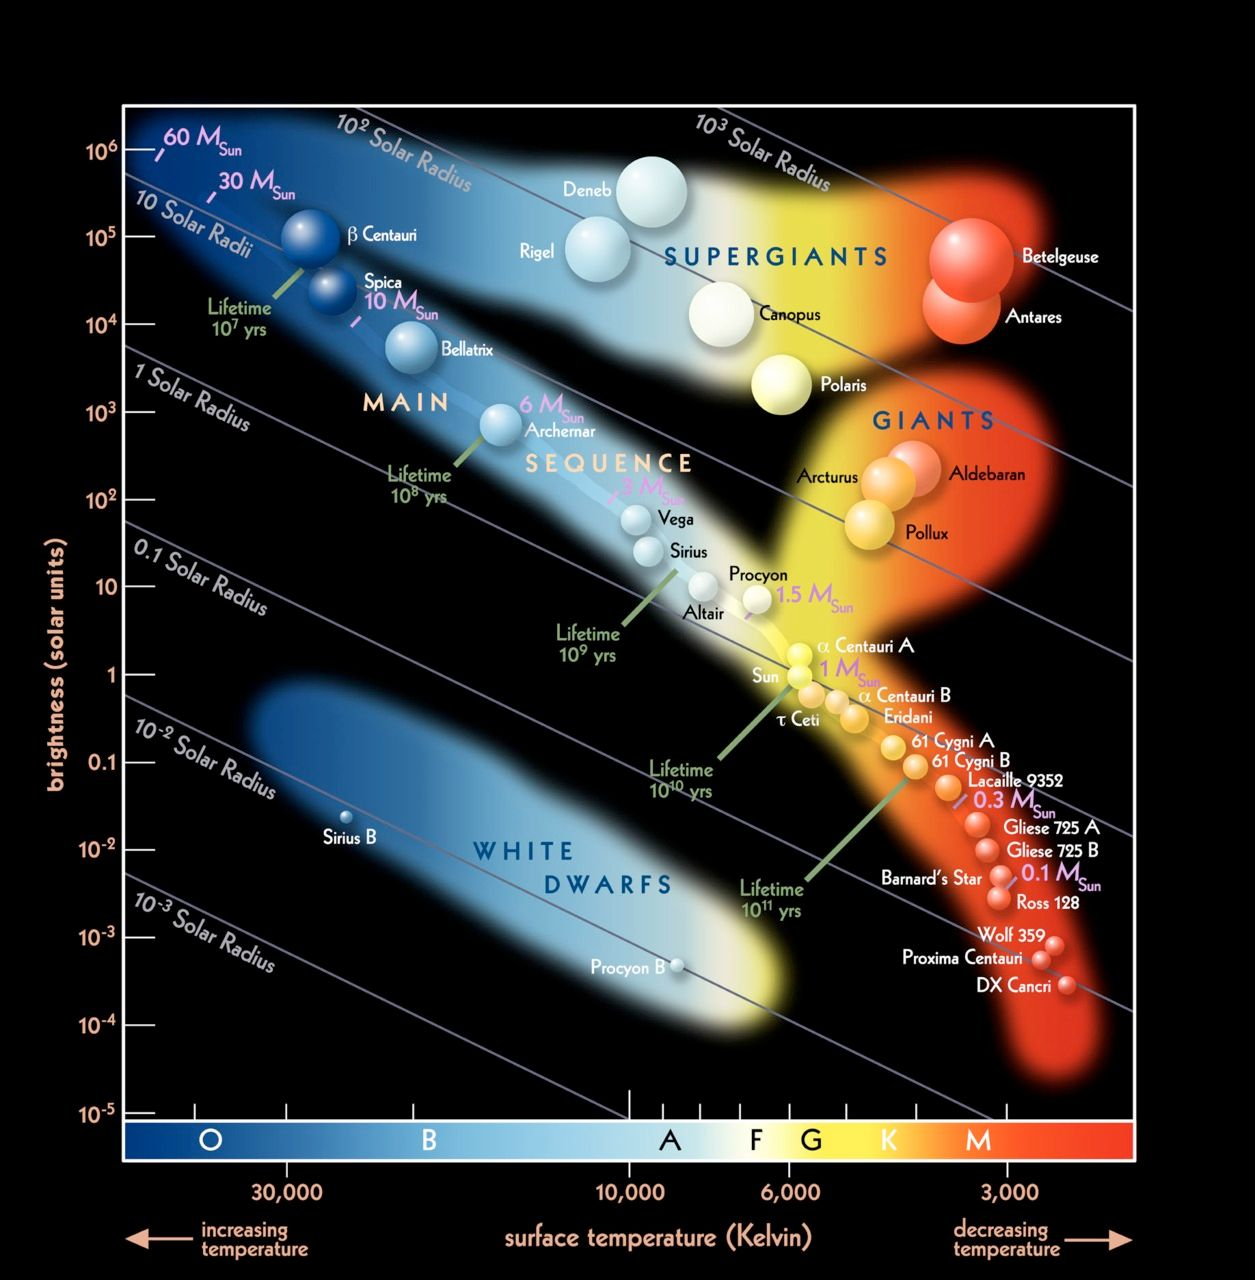
\includegraphics[width=0.65\textwidth]{images/Hertzsprung_Russel_Diagram.jpg}
    \end{center}
    \caption{WRITE CAPTION, INSERT REFERENCE}\label{fig: Hertzsprung_Russel_Diagram}
\end{figure}\\
Since almost all stars go through a phase in the MS, and evolve from there differently, in this work, the chosen starting point for stellar evolution is the Zero Age Main Sequence (ZAMS). 
At this stage, stars have just begun hydrogen burning in their cores, marking the start of their stable main sequence phase.
This allows to bypass the early phases of star formation, which are much less relevant to the gravitational wave sources of interest, while still capturing the essential evolutionary processes that lead to the formation of compact objects.

\subsection{Single star evolution}
Simulating the evolution of a single star is in itself a very complex matter, and the only way to make it computationally feasible in the context of large-scale population synthesis is to approximate the evolution for a wide range of mass $M$ and metallicity $Z$. 
In fact, detailed evolution codes can require substantial computational time even for the evolution of a single star, which is not practical when generating a full-scale astrophysical population containing millions of stars. 
Also, in order to make population synthesis statistically robust a large enough number of stars of a certain type must be evolved in order to overcome stochastic noise (in particular, the Poisson noise for $n$ simulations of a particular type of star, implies an error that grows as $\sqrt{n}$).
A winning strategy, adopted by several population synthesis frameworks, is to pre-generate a large grid of detailed stellar evolution models, and use them to derive a number of interpolation formulae as functions that approximate stellar properties as a function of age, mass and metallicity. 
In \cite{SSE} this method is implemented through the development of a set of \textbf{Single Star Evolution} (\textbf{SSE}) formulae, with the result of a very compact, efficient and adaptable code, which makes it perfect for the integration of binary-star interactions.
The work presented in \cite{SSE} therefore serves as the theoretical and computational foundation for many complex stellar population synthesis codes, including the one used in this thesis. It takes care of the single-star evolution of stars from ZAMS through all the possible evolutionary outcomes, depending on the star's initial conditions.

\subsection{Binary stars evolution}
While the evolution of single stars already represents a challenge, the inclusion of binary interactions introduces a much higher level of complexity.
In such systems, the evolution of each star is strongly influenced by its companion through a variety of processes, such as mass transfer and accretion, common envelope evolution, collisions, supernova kicks, tidal effects, angular momentum loss, and mergers.
These interactions can drastically alter the final outcomes, and are essential for modeling the formation of compact binaries that are potential gravitational wave targets for LISA.
To efficiently model binary evolution within the framework of stellar population synthesis, the work of \cite{BSE} extends the SSE formalism by introducing a set of prescriptions for binary interactions, and updating the treatment of processes such as Roche lobe overflow, common envelope evolution ans coalescence by collision, leading to the development of the \textbf{Binary Star Evolution} (\textbf{BSE}) algorithm.
This code includes the interpolation-based approach used in SSE for single-star evolution, but adds a comprehensive treatment of binary-specific processes, enabling the simulation of a wide range of binary configurations but keeping the affordable computational requirements of SSE.
The BSE algorithm tracks the joint evolution of both stars in a binary system, taking into account their initial parameters, such as masses, orbital period, eccentricity, and metallicity, and updates these properties dynamically as the system evolves.
The flexibility and speed of the BSE code make it a key component in many modern population synthesis tools, including the one used in this thesis, which we will now introduce.

\section{COSMIC}
For the purposes of this work, we employ a community-developed binary population synthesis (BPS) python-based code, called the \textbf{Compact Object Synthesis and Monte Carlo Investigation Code} (\textbf{COSMIC}), whose <<\textit{primary purpose is to generate synthetic populations with an adaptive size based on how the shape of binary parameter distributions change as the number of simulated binaries increases}>>
\footnote{\url{https://cosmic-popsynth.github.io/docs/stable/pages/about.html}}. 
COSMIC's binary evolution is built upon BSE, incorporating extensive modifications in order to include updated physical prescriptions.
It  includes all necessary tools to generate a population, from the generation of initial conditions, to scaling the simulated systems to full-scale astrophysical populations.
The code is presented in \cite{Breivik}, where it is described in full detail and used, as a proof of concept, to simulate the Galactic population of compact binaries and their associated gravitational wave signal.
In the following section we will see the main features of the code, and explain what makes it the right choice for this thesis work.

\subsection{Fixed population}
A fundamental concept in COSMIC, which is the key to the code's efficiency, is the idea of \textit{fixed population}.
This refers to a relatively small sample\footnote{Note that, from now on, every time we talk about sampling, that is where the "M" of COSMIC comes into play: this code uses proficiently the Monte Carlo Markov Chain methods to sample populations and parameter distributions, as will follow in this section.} of just enough binaries to capture, in a statistically meaningful way, the underlying shape of the parameter distribution functions of the target population, as determined by the user specified Star Formation History (SFH) and evolution model.
This is achieved following an iterative process designed to reach a convergence with respect to a defined matching condition, and consists of five key steps:
\begin{enumerate}
    \item The user selects a binary evolution model and SFH;
    \item Based on the SFH and the chosen initial parameter distribution, an initial population is generated;
    \item The population evolves for a user specified number of steps, according to the selected evolution model;
    \item If it is the first iteration, half of the simulated systems is compared with the total population. In the following steps, the population from the previous one gets compared to the population containing both the current and previous iterations.
    In any case, the comparison is done in order to check if the matching condition has been achieved;
    \item Once the parameter distributions of the population have converged, the corresponding population is called \textit{fixed population}, which represents the statistical features of a binary evolution model.
\end{enumerate}
In practice, the fixed population is the converged, computationally efficient representation of the systems that we want to simulate, embedded in a complete small-scale synthetic galaxy that also contains other stellar components.
The output is stored in a data frame, which separates the full galaxy properties from the fixed population ones.
The last step required to construct a full size galaxy is to scale the fixed population (by mass or by number of stars) with a re-sampling approach with replacement, allowing to extrapolate a larger final population that preserves the statistical properties encoded in the fixed population.

\subsubsection{Initialization}
The fixed population is generated from an initial collection of binaries sampled from distribution functions to assign to each binary an initial value of metallicity ($Z$), primary star mass ($m$), mass ratio ($q$), orbital separation ($a$), eccentricity ($e$), and birth time ($T_0$) according to the selected SFH.
In COSMIC the user can choose between different binary parameter distributions, and different parameters can be treated independently.
%In particular:
% \begin{itemize}
%     \item Masses can be sampled from the \cite{Salpeter}, \cite{Kroupa93} or \cite{Kroupa01} Initial Mass Function (IMF);
%     \item Mass ratios are uniformly sampled from \cite{Mazeh92} and \cite{Mazeh94};
%     \item Orbital separations are log-uniformly sampled following \cite{Dominik};
%     \item Eccentricities can be sampled from \cite{Heggie} or from \cite{Geller}; 
%     \item Binarity can follow \cite{Haaften} or follow user specified fractions; 
%     \item COSMIC can also generate initial binary samples following \cite{MoeDiStefano}.
% \end{itemize}
% In this thesis we chose to have independent parameter distributions, and used the default options for all of them, which means \cite{Kroupa01} for the primary model, COMPLETE THIS PART.
Moreover, COSMIC allows a complete personalization of the initial population through a number of other parameters, including different time-steps to control the binary physics, metallicity, stellar winds, common envelope phase, natal kicks, remnant mass, remnant spin, gravitational wave orbital decay, mass transfer, tides, and particular specifications for different kinds of stellar objects, mixing variables, and magnetic braking.
In this work all the parameters were left default, but one: we tweaked the metallicity value, in order to differentiate fixed populations describing the parameter distributions for galaxies of different types.
We will go more into detail on this topic in the next chapters.

\subsubsection{Convergence}
The number of simulated systems in the fixed population ideally describes the final parameter distribution functions while being low enough to keep the code efficient. 
Since every population depends on a different binary evolution model, to quantify this number a \textit{discrete match criteria} is developed, based on the work \cite{Chatziioannou17}.
Independently generated histograms for each parameter are used to track their distribution as successive populations are generated and cumulatively added to the fixed population.
The physical limits of the simulated systems are then enforced by taking the logistic transform, and finally the match is defined as: 
\begin{equation}
    match=\displaystyle\frac{\sum_{k=1}^{N}P_{k,i} P_{k,i+1}}{\sqrt{\sum_{k=1}^{N}(P_{k,i}P_{k,i})\sum_{k=1}^{N}(P_{k,i}P_{k,i+1})}},
    \label{eq: match condition}
    \notag
\end{equation}
where $P_{k,i}$ is the probability for the \textit{k}th bin, for the \textit{i}th iteration.
For how it is defined, the match value shifts between $0$ and $1$, and tends to unity as the parameter distributions converge to a distinct shape.

\subsubsection{The output}
Since COSMIC uses BSE as it’s core binary evolution algorithm, the output of COSMIC follows most of the same conventions as BSE. The \textit{kstar values} (e.g. the number that represent a specific stellar type) and evolution stages are nearly identical to their BSE counterparts, and the exact references can be found in the \textbf{Appendix}.
In order to generate a fixed population, the COSMIC can be ran through a one-line command directly on the terminal, specifying a parameter file, the kstar values for the primary and secondary star, the maximum number of systems to evolve, every how many systems to check in, in order to track the distributions of the parameters, and how many processors to use.
The final output is in an \textit{hdf5} file containing several data frames, that keep track pf various important quantities during the evolution: the total number of stars and total mass of the entire population, the number of binaries, the convergence, and so on. 
The \textit{conv} data frame contains all the information about the final fixed population, and thus is the one that we will use the most: from it we can extract all the parameter distributions of the fixed population, such as the orbital parameters, and the individual star information.
The parameter distributions of a fixed population of binary white dwarfs with a default metallicity value set at $0.020$ is shown in \textbf{Figure~\ref{fig: first fixed pop distributions}}.
\begin{figure}[ht!]
    \begin{center}
        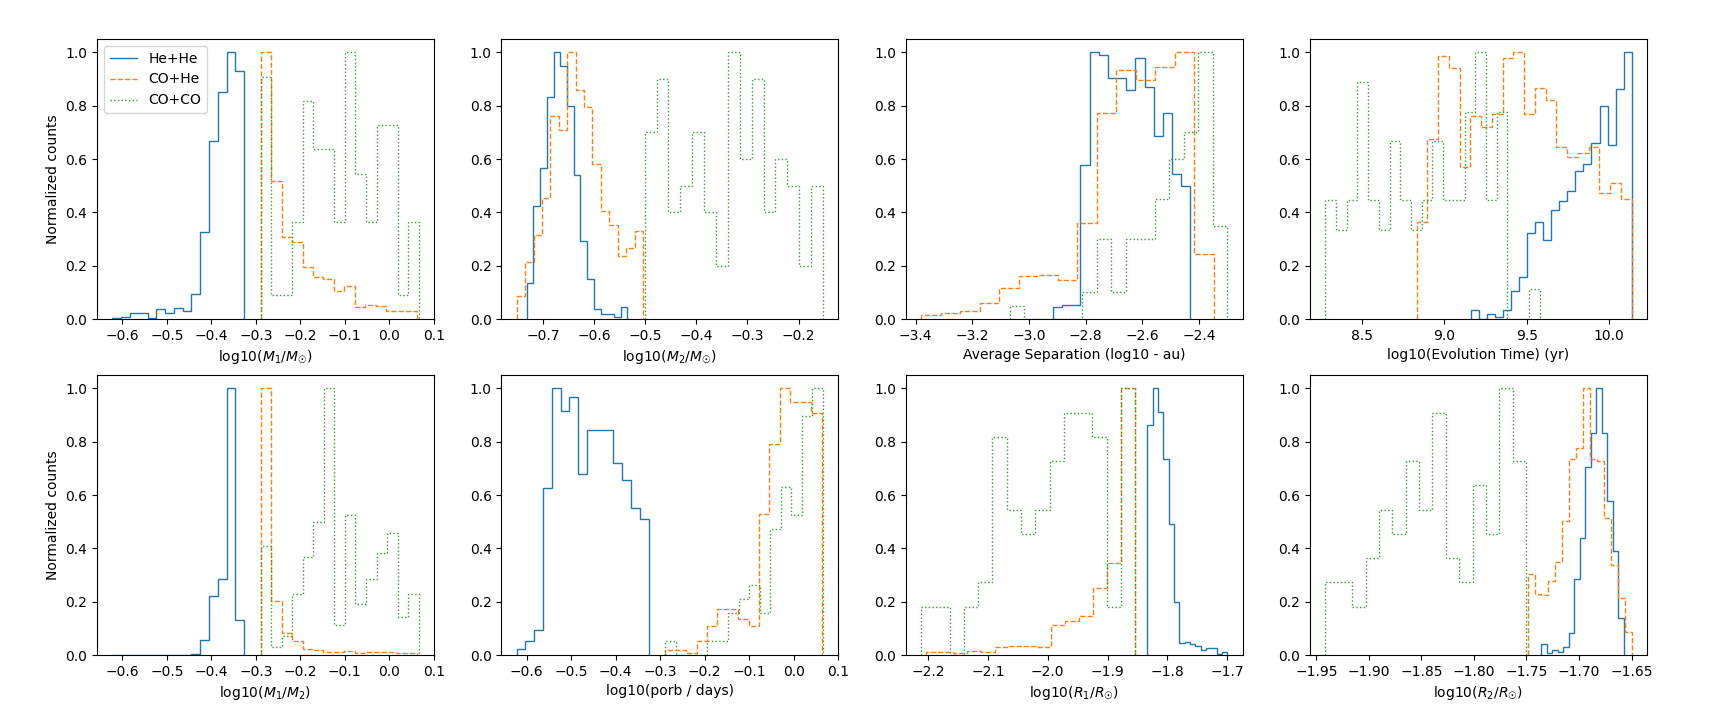
\includegraphics[width=0.85\textwidth]{images/first_fixed_params_distr.jpg}
    \end{center}
    \caption{Distributions of the parameters of a fixed population with metallicity $Z=0.020$ composed of He+He, CO+He and CO+CO binary white dwarfs. This includes the mass, radius of primary and secondary stars, the radius ratios between the two, the orbital period, average separation, and evolution time.}\label{fig: first fixed pop distributions}
\end{figure}



\subsection{Astrophysical population}
Once the convergence criteria is achieved, an astrophysical population can be sampled. 
The number of sources in the astrophysical population $N_{astro, tot}$ can be found by upscaling the size of the fixed population, $N_{fixed}$ ,by the ratio of the mass of the astrophysical population, $M_{astro}$, to the mass of all the stars in the whole small-scale galaxy in which the fixed population is embedded, $M_{fixed,stars}$, as follows:
\begin{equation}
    N_{astro} = N_{fixed}\frac{M_{astro, tot}}{M_{fixed, stars}},
    \label{eq: scale by mass}
\end{equation}
or by the ratio of the number of stars in the astrophysical
population, $N_{astro, tot}$, to the total number of stars formed to produce the fixed population, $N_{fixed,tot}$,
\begin{equation}
    N_{astro} = N_{fixed}\frac{N_{astro, tot}}{N_{fixed, stars}}.
    \label{eq: scale by number}
\end{equation}
Thus, to create a full-scale astrophysical population we need a \textit{reference population} from which we can extract either the total mass or the total number of stars, to then use to scale up our fixed population.
As we will now see, the chosen reference for our purpose is a catalog which reports many key galactic parameters in it, which will allow us to proceed using the method in \eqref{eq: scale by mass}.



\section{GWGC and Galaxy Properties}
As we have seen, the goal of this work is to simulate the gravitational wave background produced by compact binaries in the \textit{local universe}, by generating the sources using COSMIC.
To replicate the existing, observed galaxies in the vicinity of the Milky Way and simulate their stellar content we rely on the dataset provided in \cite{GWGC}, the \textbf{Gravitational Wave Galaxy Catalog} (\textbf{GWGC}).
This catalog includes a list of $53,255$ galaxies within $100Mpc$ from earth, containing information on sky position, distance, blue magnitude, major and minor diameters, position angle, and galaxy type, currently used for follow-up searches of electromagnetic counterparts from gravitational wave searches.

\subsection{What it has vs what we need}
In principle, we could generate a separate fixed population for each galaxy in the GWGC and scale it individually.
However, this is simply not practical because of the computational power and time it would require, and therefore we must find a strategy to group them in a few, representative, categories.
As we will show in this section, many of the information in the GWGC can be used to infer the missing astrophysical quantities we need for population synthesis. 
Ultimately, we will find that metallicity is the most suitable parameter for grouping galaxies.
To get there, we follow a chain of empirical relations, starting from the galaxy morphological type, through  a luminosity to mass, and then a mass to metallicity relation. 
This process will enable us to provide COSMIC with the necessary input, found in a consistent and astrophisically motivated way.

\subsection{Galaxy types}

    - T value to Class

\subsection{Mass-luminosity relation}

    - Class to Mass-Luminosity relation -> Mass (Faber \& Gallagher)

\subsection{Mass-metallicity relation}

    - Finding each galaxy's metallicity from the mass (Tremonti - Allende Prieto)


\section{The final fixed populations}

\subsection{Final catalog editing}

    - Graphs of catalog distributions

\subsection{Metallicity categorization}

    - Metallicity bins for GWGC galaxies, and corresponding fixed populations


\section{Total Gravitational Wave Signal}
- For each galaxy:
    - Compute right $N_astro$
    - compute each binary's GW signal;
    - bin it to LISA's frequency sensibility bins
    - Plot it on LISA's sensibility curve
- Zone of avoidance: how to consider all the sky


